\chapter{Testowanie Contiguous Memory Allocatora}

Aby sprawdzić działanie alokatora \acc{CMA}, w~tym rozdziale opiszę
jak go przetestować na przykładzie laptopa \acc{MSI} U100 z~jednym
\unit{GiB} pamięci \acc{RAM} z~zainstalowanym systemem Slackware 14.0.
Do testów wybrałem tę dystrybucję \acc{GNU}/Linuksa, gdyż jest ona
stosunkowo prosta w~użyciu, a~jednocześnie pozostaje wierny filozofii
Uniksa, dzięki czemu łatwo jest wymieniać komponenty systemu takie jak
jądro.


\section{Instalacja jądra z~obsługą \acc{CMA}}

Standardowo Linux nie posiada obsługi alokatora \acc{CMA}, dlatego
pierwszym krokiem będzie zmiana jądra systemu na wersję 3.5
z~włączonym mechanizmem \acc{CMA}.  Wymagane źródła można pobrać ze
strony \url{http://kernel.org/}, która jest głównym miejscem
dystrybucji Linuksa.

Przed kompilacją jądra należy je najpierw skonfigurować.  Aby ułatwić
ten proces, zamiast ustawiać wszystko od początku, warto skorzystać
z~już istniejącego pliku konfiguracyjnego.  Zazwyczaj konfiguracja
obecnie uruchomionego jądra jest dostępna w~pliku
\code{/proc/config.gz}\footnote{W~dystsrybucjach innych niż Slackware
  plik ten może byc nieobecny.  W~takim przypadku należy sprawdzić
  obecność pliku \code{/proc/config}.  Jeżeli również i~ten plik nie
  jest dostępny, warto poszukać plików których nazwa rozpoczyna się od
  \code{config} w~katalogu \code{/boot}.}.  Aby uruchomić program
konfiguracji jądra, należy wykonać następującą sekwencję poleceń:

\begin{lstlisting}[language=sh,numbers=none]
wget http://www.kernel.org/pub/linux/kernel/v3.0/linux-3.5.tar.xz
xz -d <linux-3.5.tar.xz | tar xf
cd linux-3.5
gzip -d </proc/config.gz >.config
make xconfig
\end{lstlisting}

Uruchomi to graficzny interfejs użytkownika, który pozwala wybrać
opcje z~jakimi jądro ma zostać zbudowane.  W~przypadku kompilacji
w~środowisku tekstowym, zamiast polecenia \code{make xconfig} należy
wykonać komendę \code{make menuconfig}, które uruchomi interfejs
tekstowy oparty o~bibliotekę ncurses.

Aby móc testować \acc{CMA} należy w~nim zaznaczyć opcje \ang*{Prompt
  for development and/or incomplete code/drivers} w~sekcji
\ang*{General setup} (zob.\ rys.\ \subref*{fig:xconfig-exp}) oraz
\ang*{Contiguous Memory Allocator} w~sekcji \ang*{Device Drivers
  $\rightarrow$ Generic Driver Options}
(zob.\ rys.\ \subref*{fig:xconfig-cma}).  Ponadto, aby umożliwić
dalsze testy należy również upewnić się, że opcja \ang*{Enable
  loadable module support} jest wybrana\,---\,bez tej opcji nie będzie
możliwe zbudowanie ani załadowanie modułu testowego opisanego
w~następnym podrozdziale.

\begin{figure}[tbp]
  \centering
  \subfloat[Opcja umożliwiająca wybór eksperymentalnych funkcji jądra.]{
    \label{fig:xconfig-exp}
    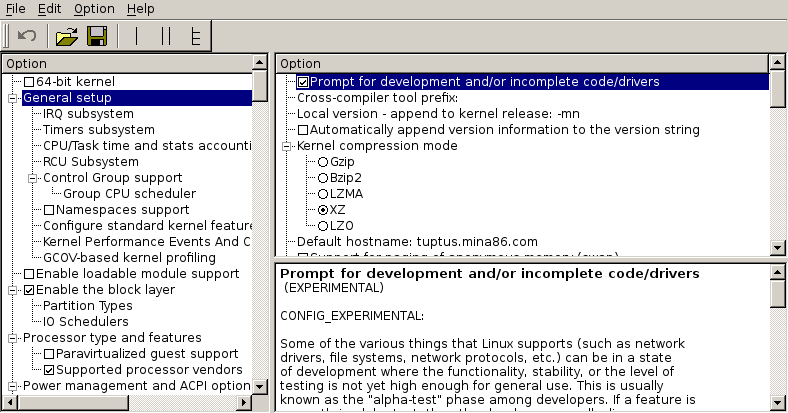
\includegraphics[width=.9\textwidth]{build/xconfig-exp.eps}
  }
  \vspace{\baselineskip}
  \subfloat[Opcja włączająca \acc{CMA}.]{
    \label{fig:xconfig-cma}
    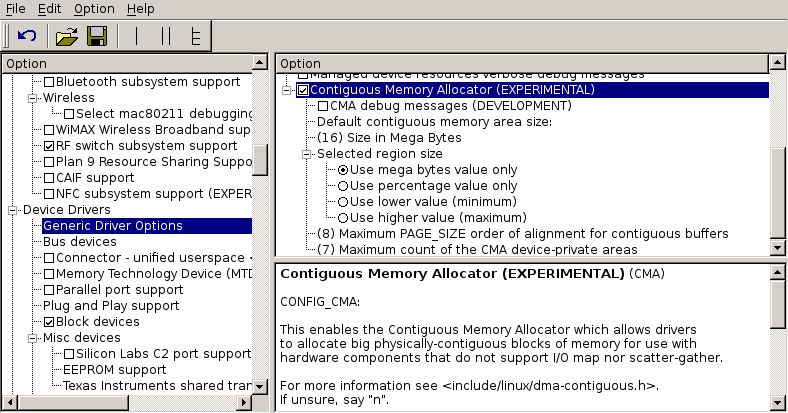
\includegraphics[width=.9\textwidth]{build/xconfig-cma.eps}
  }
  \caption{Graficzny interfejs konfiguracji jądra.}
  \label{fig:xconfig}
\end{figure}

W~przypadku jakichkolwiek problemów ze znalezieniem danej opcji, warto
skorzystać z~funkcji wyszukiwania wbudowanej w~program konfiguracyjny.
Aktywuje się ją wciśnięciem sekwencji klawiszy Ctrl+F (lub w~przypadku
tekstowego interfejsu \code{menuconfig} poprzez wciśnięcie przycisku
slash).

Gdy konfiguracja zostanie zakończenie należy zbudować i~zainstalować
nowe jądro zgodnie z~opisem w~\autocite{bib:building-linux}.  Aby móc
testować alokator \acc{CMA}, należy ponadto stworzyć dodatkowe wpisy
w~\code{/etc/lilo.conf} różniące się opcją \code{append}, która
powoduje, że program startujący przekazuje dodatkowe opcje do jądra:

\begin{itemize}
\item \code{append = "cma=0"} wyłączy \acc{CMA} tak, że jądro będzie
  zachowywać się jakby obsługa \acc{CMA} nie była dostępna.
\item \code{append = "cma=0 mem=512m"} spowoduje, że Linux będzie
  korzystał tylko z~pierwszych \unit[512]{MiB} pamięci \acc{RAM}.  Ustawienie
  to pozwala symulować sytuację, w~której część pamięci jest na stałe
  zarezerwowane dla sterowników.
\item \code{append = "cma=512m"} skonfiguruje alokator \acc{CMA}, tak aby
  zarezerwował pojedynczy region rozmiaru \unit[512]{MiB} do
  wykorzystania dla sterowników.
\end{itemize}

Po uruchomieniu nowego jądra, obecność mechanizmu \acc{CMA} można
sprawdzić analizując plik \code{/proc/pagetypeinfo}.  Zawiera on
statystyki alokatora stron w~postaci liczby stron różnych typów
w~poszczególnych strefach.  Jeżeli alokator \acc{CMA} jest obecny
w~jądrze plik ten posiada linie zawierające nazwę \code{CMA}, które
informują ile stron \acc{CMA} jest wolnych w~systemie.  Ponadto plik
\code{/proc/cmdline} zawiera pełną listę argumentów jakie program
startujący przekazał jądru.  Może on być przydatny do weryfikacji, czy
opcje są poprawnie przekazywane.


\section{Modułu testowy cma\_test}

Do testów \acc{CMA} wykorzystam moduł Barry'ego Songa.  Po nałożeniu
\autocite{patch:cma-test} na źródła jądra 3.5 powstanie nowy katalog
\code{tools/cma} z~nowym sterownikiem.  Niestety był on testowany
jedynie na architekturze \acc{ARM} i~aby zadziałał na systemie x86
należy zmodyfikować plik \code{cma_test.c} wprowadzając dwie zmiany.
Po pierwsze, zaraz po ostatniej dyrektywie \code{#include} należy
dodać następujące linie:

\begin{lstlisting}[numbers=none]
#ifndef SZ_1K
#  define SZ_1K 1024
#endif

static u64 cma_test_dma_mask = ~(u64)0;
\end{lstlisting}

Po wtóre, w~funkcji \code{cma_test_init}, tuż przed linią przypisującą
wartość do pola \code{coherent_dma_mask} obiektu \code{cma_dev},
należy dodać linijkę:

\begin{lstlisting}[numbers=none]
	cma_dev->dma_mask = &cma_test_dma_mask;
\end{lstlisting}

Po wprowadzeniu tych modyfikacji moduł można skompilować wykonując
polecenie \code{make} wewnątrz katalogu \code{tools/cma}, w~wyniku
czego powstanie plik \code{cma_test.ko}.  Całą operację (łącznie
z~pobieraniem i~dodaniem źródeł modułu do jądra) można sprowadzić do
wykonania sekwencji poleceń z~wydruku \ref{lst:compile-cma-test}
w~katalogu ze źródłami Linuksa.

\begin{lstlisting}[float=tb,caption=Sekwencja komend dodająca
    i~budująca moduł \code{cma_test}.,
    label=lst:compile-cma-test,language=sh,numbers=none]
wget -O cma_test.patch https://patchwork.kernel.org/patch/1158071/raw/
patch -p1 <cma_test.patch
cd tools/cma
sed -i -e '/struct cma_allocation {/ i\
#ifndef SZ_1K\
#  define SZ_1K 1024\
#endif\
\
static u64 cma_test_dma_mask = ~(u64)0;\
\
/coherent_dma_mask/ i	cma_dev->dma_mask = &cma_test_dma_mask;' \
    cma_test.c
make
\end{lstlisting}

Po wczytaniu modułu poleceniem \code{insmod cma_test.ko} w~systemie
pojawi się urządzenie \code{/dev/cma_test}, które służy do wykonywania
testowych alokacji z~wykorzystaniem interfejsu \acc{DMA} \acc{API}
(a~zatem pośrednio z~użyciem alokatora \acc{CMA}).  Zapis do tego
pliku liczby naturalnej spowoduje wykonanie alokacji podanej liczby
kibibajtów, a~odczyt zwolnienie najwcześniej zaalokowanego obszaru.

Przykładowo, wykonanie polecenia \code{echo 1024 >/dev/cma_test}
spowoduje alokację bufora o~rozmiarze jednego mebibajta, gdy tymczasem
polecenie \code{cat /dev/cma_test} spowoduje zwolnienie tego bufora.


\section{Testowanie alokacji pamięci}

Aby zobaczyć efekt działania opcji \code{mem} oraz mechanizmu
\acc{CMA} wykorzystać można prosty program \code{malloc} przedstawiony
na wydruku \ref{lst:malloc}.  Nie robi on nic poza żądaniem pamięci
w~pętli.  Linux domyślnie opóźnia alokację pamięci do pierwszej próby
modyfikacji, dlatego program musi zapisać coś w~zaalokowanej stronie.

\lstinputlisting[float=tb,caption=Prosty program testujący alokację
  pamięci.,label=lst:malloc]{code/malloc.c}

Po uruchomieniu program będzie działał w~kółko żądając coraz więcej
pamięci do momentu, gdy jądro nie będzie już w~stanie zaspokoić tych
żądań.  Wówczas \ang*{out-of-memory killer} wymusi zakończenie
programu.  Jest to mechanizm jądra, którego celem jest
zagwarantowanie, iż system zawsze będzie miał pewne rezerwy wolnej
pamięci.

Uruchomiony na systemie z~jednym \unit{GiB} pamięci program zakończył
się po zaalokowaniu około \unit[965]{MiB}, gdy mechanizm \acc{CMA} był
wyłączony, oraz \unit[964]{MiB}, gdy na potrzeby \acc{CMA} było
zarezerwowane \unit[512]{MiB}.  Różnica jednego megabajta jest
pomijalna i~wskazuje, iż istotnie pamięć rezerwowana przez \acc{CMA}
jest dostępna dla systemu.

Jednocześnie gdy jądro wystartowało z~opcją \code{mem=512m}, program
został zatrzymany po zaalokowaniu \unit[477]{MiB}.  Pokazuje to
w~praktyce działanie argumentu \code{mem} jądra.

Podobnie gdy system wystartował z~regionem \acc{CMA} o~rozmiarze
\unit[512]{MiB}, a~następnie dokonano alokacji tej pamięci poprzez
czterokrotne wykonanie polecenia \code{echo 131072 >/dev/cma_test},
program \code{malloc} ponownie nie był w~stanie zaalokować więcej niż
\unit[454]{MiB} pamięci.  Spowodowane to było rzecz jasna tym, iż
sterownik \code{cma_test} trzymał połowę pamięci i~jądro miało do
dyspozycji jedynie \unit[512]{MiB}.

Ilość pamięci, którą udało się zaalokować programowi \code|malloc|
przy różnych ustawieniach jądra oraz różnych buforach zaalokowanych
z~puli \acc{CMA} przedstawia tablica \ref{tab:cma-test-allocs}.
Kolumna „\code|append|” tej tablicy określa parametry przekazane do
jądra, kolumna „Alokacja \acc{CMA}” określa jaki rozmiar pamięci
\acc{CMA} został zaalokowany przez moduł testowy \code{cma_test},
a~kolumna „Udana alokacja” wskazuje ile pamięci udało się zaalokować
programowi \code{malloc} zanim system wymusił jego zakończenie.

\begin{table}[tbp]
\begin{center}
\begin{tabular}{llrr}
    & \code|append|         & Alokacja \acc{CMA} & Udana alokacja \\
\hline
(1) & \code|cma=0|          &                   & \unit[965]{MiB} \\ % 988284
(2) & \code|cma=512m|       &     \unit[0]{MiB} & \unit[964]{MiB} \\ % 987628
(3) & \code|cma=512m|       &   \unit[128]{MiB} & \unit[837]{MiB} \\ % 857428
(4) & \code|cma=512m|       &   \unit[256]{MiB} & \unit[710]{MiB} \\ % 726804
(5) & \code|cma=512m|       &   \unit[384]{MiB} & \unit[582]{MiB} \\ % 596108
(8) & \code|cma=512m|       &   \unit[512]{MiB} & \unit[455]{MiB} \\ % 465420
(7) & \multicolumn{2}{l}{\code|cma=0 mem=512m|} & \unit[477]{MiB} \\ % 488900
\end{tabular}
\end{center}
\caption[Ilość zaalokowanej z~sukcesem pamięci.]{Ilość pamięci
  zaalokowanej z~sukcesem na testowym systemie z~jednym \unit{GiB}
  pamięci.}
\label{tab:cma-test-allocs}
\end{table}


\section{Testowanie szybkość działania systemu}

Aby zmierzyć jak zmniejszona ilość dostępnej pamięci może wpływać na
szybkość systemu posłużę się programem \code{seq_read} zaprezentowanym
na wydruku \ref{lst:seq-read}.  Jego działanie sprowadza się do
sekwencyjnego odczytu podanego pliku\footnote{Należy zauważyc, że
  program odczytuje jedynie pierwszy bajt z~każdych \unit[4]{KiB}
  zadanego pliku.  Ponieważ wykorzystana jest funkcja \code|mmap|
  wymusza to wczytanie całego bloku do pamięci, jednak jeżeli strona
  posiada już potrzebne dane, odczyt jest szybszy niż odczyt całej
  strony z~pamięci RAM.  Program \code|seq_read| jest napisany w~ten
  sposób, aby uwypuklić efekty buforowania.} i przyjmuje trzy
argumenty:

\begin{enumerate}
\item Nazwę pliku, który ma być odczytany.  Musi to być zwykły plik,
  którego rozmiar jest nie mniejszy niż jedna strona (\unit[4096]{B}).
\item Opcionalną liczbę określającą ile razy plik ma być odczytany.
  Wielokrotny odczyt pozwala z~większą dokładnością zmierzyć ile czasu
  zajmuje pojedynczy odczyt.  Jeżeli argument ten nie jest podany,
  plik zostanie odczytany tylko raz.
\item Opcjonalną liczbę określającą maksymalny rozmiar pliku.  Jeżeli
  argument jest podany i~jest mniejszy od rozmiaru pliku, tylko podana
  liczba bajtów będzie brana pod uwagę.  Pozwala to testować różne
  rozmiary plików stosując tylko jeden duży plik.
\end{enumerate}

Przeprowadzone przeze mnie testy polegały na zmierzeniu ile czasu
zajmie programowi \code|seq_read| odczyt pliku najpierw raz, a~potem
sto razy.  Oba wywołania programu wykonałem dla różnych wartości
argumentu \code|append| (przekazywanego przez \acc{LILO} do jądra)
oraz z~różnym rozmiarem zaalokowanych buforów \acc{CMA}, za każdym
razem restartując system.  Do zautomatyzowania tego procesu,
posłużyłem się skryptep \code|run_test.sh| przedstawiony na wydruku
\ref{lst:run-test}.  Do poprawnego działania wymaga obecności pliku
\code|rand-1g| o~rozmiarze przynajmniej jednego \unit[GiB], który
można stworzyć za pomocą następującej sekwencji poleceń:

\begin{lstlisting}[language=sh,numbers=none]
head -c 4096 /dev/urandom >rand
for i in $(seq 18); do cat rand rand >tmp && mv tmp rand; done
mv -- rand rand-1g
\end{lstlisting}

Pierwsze dwa argumenty skryptu \code|run_test.sh| mają takie samo
znaczenie jak drugi i~trzeci argument programu \code|seq_read|, tyle
że maksymalna wielkość podana jest w~mebibajtach, a~nie w~bajtach.
Ponadto, trzeci argument, jeżeli jest podany, określa ile bloków
rozmiaru \unit[128]{MiB} ma być zaalokowanych przez moduł
\code|cma_test| przed uruchomieniem testów.  Aby ta opcja działała
poprawnie program musi być uruchomiany z~konta użytkownika \code|root|
oraz albo moduł \code|cma_test| musi być wczytany, albo plik
\code|cma_test.ko| dostępny.

Dzięki uruchomieniu programu \code|seq_read| poprzez polecenie
\code|time|, automatycznie następuje pomiar czasu.  Po zakończeniu obu
wywołań programu \code|seq_read| skrypt \code|run_test.sh| czeka na
wciśnięcie klawisza Enter, po czym restartuje system (aby temu
zapobiec, wystarczy zamiast Enter wcisnąć Ctrl+D).

\lstinputlisting[float=tb,caption=Skrypt \code|run_test.sh| służący do
  wykonywania pojedynczej iteracji testu.,
  label=lst:run-test,language=sh]{code/run_test.sh}

\lstinputlisting[float=tb,caption=Prosty program sekwencyjnie
    odczytujący plik.,label=lst:seq-read]{code/seq_read.c}

Tablica \ref{tab:seq-read-times-first} przedstawia czas jaki był
potrzebny do jednorazowego odczytanie zadanej liczby mebibajtów pliku.
Zgodnie z~przewidywaniami, ponieważ zaraz po uruchomieniu komputera
system nie miał szansy buforować pliku, liczba dostępnej pamięci nie
wpływa na czas działania programu\,---\,za każdym razem jądro musi
bowiem wczytać cały plik.

\begin{table}[tbp]
  \centering
  \begin{tabular}{llrrrr}
    & & & \multicolumn{3}{c}{Czas pierwszego odczytu} \\
    & \code|append|        & Alokacja \acc{CMA} & \unit[300]{MiB} & \unit[600]{MiB}  & \unit[900]{MiB}  \\
\hline
(1) & \code|cma=0|            &                 & \unit[5,925]{s} & \unit[11,598]{s} & \unit[17,426]{s} \\
(2) & \code|cma=512m|         &   \unit[0]{MiB} & \unit[5,839]{s} & \unit[11,685]{s} & \unit[17,537]{s} \\
(3) & \code|cma=512m|         & \unit[128]{MiB} & \unit[5,844]{s} & \unit[11,798]{s} & \unit[17,554]{s} \\
(4) & \code|cma=512m|         & \unit[256]{MiB} & \unit[5,803]{s} & \unit[11,701]{s} & \unit[17,645]{s} \\
(5) & \code|cma=512m|         & \unit[384]{MiB} & \unit[5,764]{s} & \unit[11,726]{s} & \unit[17,456]{s} \\
(6) & \code|cma=512m|         & \unit[512]{MiB} & \unit[5,885]{s} & \unit[11,773]{s} & \unit[17,449]{s} \\
(7) & \multicolumn{2}{l}{\code|cma=0 mem=512m|} & \unit[5,701]{s} & \unit[11,784]{s} & \unit[17,627]{s} \\
  \end{tabular}
  \caption[Czas odczytu pliku „na zimno”.]{Czas potrzebny do
    odczytania podanej liczby mebibajtów pliku zaraz po restarcie
    systemu.}
  \label{tab:seq-read-times-first}
\end{table}

O~wiele ciekawsza jest tablica \ref{tab:seq-read-times-nth}, która
pokazuje ile czasu zajął pojedynczy odczyt po zakończeniu wstępnego
odczytu.  W~przypadku, gdy w~systemie jest dużo wolnej pamięci, jądro
jest w~stanie trzymać cały plik w~pamięci, dzięki czemu kolejne
odczyty są bardzo szybkie i~nawet odwołanie się do \unit[900]{MiB}
zajmuje niecałe cztery setne sekundy.

\begin{table}[tbp]
  \centering
  \subfloat[Tablica z~czasem.]{
    \label{tab:seq-read-times-nth:sub}
    \begin{tabular}{llrrrr}
    & & & \multicolumn{3}{c}{Czas kolejnych odczytów} \\
    & \code|append|        & Alokacja \acc{CMA} & \unit[300]{MiB} & \unit[600]{MiB}  & \unit[900]{MiB}  \\
\hline
(1) & \code|cma=0|            &                 & \unit[0,011]{s} & \unit[ 0,023]{s} & \unit[ 0,035]{s} \\
(2) & \code|cma=512m|         &   \unit[0]{MiB} & \unit[0,011]{s} & \unit[ 0,024]{s} & \unit[ 0,037]{s} \\
(3) & \code|cma=512m|         & \unit[128]{MiB} & \unit[0,012]{s} & \unit[ 0,029]{s} & \unit[17,117]{s} \\
(4) & \code|cma=512m|         & \unit[256]{MiB} & \unit[0,011]{s} & \unit[ 0,024]{s} & \unit[16,941]{s} \\
(5) & \code|cma=512m|         & \unit[384]{MiB} & \unit[0,012]{s} & \unit[ 9,211]{s} & \unit[17,094]{s} \\
(6) & \code|cma=512m|         & \unit[512]{MiB} & \unit[0,012]{s} & \unit[11,633]{s} & \unit[17,382]{s} \\
(7) & \multicolumn{2}{l}{\code|cma=0 mem=512m|} & \unit[0,012]{s} & \unit[11,640]{s} & \unit[17,368]{s} \\
    \end{tabular}
  }
  \vspace{\baselineskip}
  \subfloat[Graficzna reprezentacja danych.  Oś y jest w~skali
    logarytmicznej.  Numery na osi x~odpowiadają wierszom tablicy
    \subref{tab:seq-read-times-nth:sub}.]{
    \label{fig:seq-read-times-nth}
    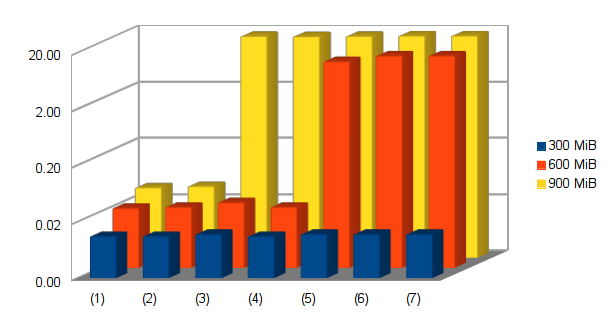
\includegraphics[width=.9\textwidth]{build/seq-read-times.eps}
  }
  \caption[Czas odczytu pliku, gdy dane były już raz odczytane.]{Czas
    potrzebny do odczytania podanej liczby mebibajtów pliku, gdy dane
    już były raz odczytane.}
\label{tab:seq-read-times-nth}
\end{table}

Gdy ilość pamięci, którą system może przeznaczyć na bufory dyskowe
maleje, czas odczytu gwałtownie rośnie.  Gdy zaledwie \unit[128]{MiB}
zostanie zaalokowanych przy użyciu mechanizmu \acc{CMA} (wiersz (3)
tablicy \ref{tab:seq-read-times-nth}), odczyt \unit[900]{MiB} „skacze”
do około 17 sekund, czyli czasu podobnego do tego potrzebnego do
odczytu pliku „na zimno”.  Wynika to z~faktu, że kolejne odczytywane
strony „wyrzucają” z~pamięci wcześniejsze strony pliku przez co, gdy
program ponownie zaczyna odczytywać plik od początku, dane nie
znajdują się już w~pamięci.

Również ciekawe jest zachowanie systemu, gdy moduł \code|cma_test|
zaalokuje \unit[384]{MiB}.  Jak wynika z~wiersza (5) tablicy
\ref{tab:cma-test-allocs} jądro może wówczas przezvaczyć około
\unit[582]{MiB} na bufory dyskowe.  Jest to rozmiar na tyle bliski
\unit[600]{MiB}, że przy odczycie właśnie takiego pliku widać poprawę
w~stosunku do sytuacji, gdy \unit[512]{MiB} jest zarezerwowanych przez
\acc{CMA}, niemniej „brakujące” \unit[12]{MiB} znacznie spowalnia
program \code|seq_read| z~tych samych powodów co opisane powyżej.


\section{Podsumowanie}

Testy szybkości odczytu pliku pokazują także w~jak dużym stopniu brak
wolnej pamięci może spowolnić pracę systemu.  Co prawda odczyt w~kółko
pojedynczego pliku nie jest realnym scenariuszem działania prawdziwej
aplikacji, niemniej aplikacje bazodanowe, czy programy do obróbki
multimediów często charakteryzują się losowym dostępem do dysku, który
przy małej ilości wolnej pamięci będzie odnosi na system podobny
efekt jak aplikacja \code|seq_read|.

Pokazuje to jak istotne jest, że alokator \acc{CMA} spełnia swoje
założenia i~pozwala sterownikom alokawać dużo obszory ciągłej
fizicznie pamięci, a~jednocześnie udostępnia zarezerwowaną pamięć
jądru podczas, gdy nie jest ona wykorzystywana przez żadne urządzenie.
To właśnie ta cecha mechanizmu \acc{CMA} odróżnia go od innych
rozwiązań problemu alokacji ciągłych fizycznie obszarów pamięci.
